
\section{Requirements and Design Constraints}

% we could include an intro here

\subsection{System Requirements}

To add custom content to the platform, a user must have a web browser and internet access. The user must also have access to modeling software or a means to provide 3D models to the website for upload.

To view AR content, the user must have an augmented reality (AR) device. Each device may have different system requirements. AR devices such as the HoloLens or mobile devices should operate as standalone hardware. Other AR devices may require a host computer to broadcast renderings to the device for viewing. Manufacturer details will outline minimum specifications for a host computer should it be needed.

E.g., the Meta 2 headset requires a separate computer for model rendering and device hosting. As of November 2017, the Meta 2 has one of the highest recommended specifications among popular AR headsets. As a result, the recommended setup will run contemporary AR applications smoothly and with significant support. The minimum and recommended specifications are listed in Table \ref{table:metatwosystemrequirements}.

\begin{table}[H]
	\centering
	\begin{tabular}{ | c | c | c | }
		\hline
		& Minimum & Recommended \\ \hline
		OS & Windows 10 (64 bit) & 	Windows 10 (64 bit) \\ \hline
		CPU & Intel i7-4770 & Intel i7-6700 \\ \hline
		RAM & 8GB DDR3 & 16GB DDR4 \\ \hline
		GPU & NVIDIA GTX 960 & NVIDIA GTX 970 \\ \hline
		Hard Drive & 2GB Free Space & 2GB+ Free Space \\ \hline
		I/O Ports & 1X HDMI 1.4b and 2X USB 3.0 ports & 1X HDMI 1.4b and 2X USB 3.0 ports \\ \hline
		3D Engine & Unity 5.6 or higher & Unity 5.6 or higher \\ \hline
	\end{tabular}

	\caption{Meta 2 System Requirements}
	\label{table:metatwosystemrequirements}
\end{table}

More up to date requirements can be found on the Meta 2 website at: 
\url{https://buy.metavision.com/}

\subsection{Network Requirements}

Being able to take advantage of the features in this product will need a network
that is able to easily upload and download 3D models. The user will need to have
both their computer and AR viewer configured for network access.

\subsection{Development Environment Requirements}
% What are they? Is the system supposed to be cross-platform?
\begin{itemize}
	\item Windows 10 - To be able to develop for the HoloLens.
	\item Visual Studio 2017 Enterprise with ASP.NET MVS, Azure and Unity tools.
	\item Unity Personal
	\item HoloToolkit - Unity Set of tools for HoloLens development with Unity.
	\item Assimp library - For file conversion
	\item FBX SDK - For file conversion
	\item Android Studio
\end{itemize}


\subsection{Project Management Methodology}
% The stakeholders might restrict how the project implementation will be managed.
%  There may be constraints on when design meetings will take place. There might
% be restrictions on how often progress reports need to be provided and to whom.

The Senior Design I team structure for this project was self-organized, having decided on the Agile development methodology and decided on Brady Shimp as a Scrum Master and Cheldon Coughlen as the Team Lead. The team had weekly status report meetings with our client representatives and faculty advisors, Dr. McGough and Dr. Karlsson. At these meetings the team provided progress reports and discussed any design modifications or complications moving forward.\\

The Senior Design II team structure for this project was refined from experiences, both good and bad, taken from the Senior Design I structure.  The team agreed that the Agile development methodology was too rigid and ineffective for a team with as many members and as many different times of availability as there were.  The team instead opted for a Feature Driven Development (FDD) methodology, that employed certain aspects of the Agile system that were deemed effective such as listing expected completion times for feature tasks and tracking productivity via the  project board. This switch allowed the team to diversify into two sub-teams, one for mobile application development and one for continued web development, that each maintained structure and accountability within themselves.  The decided leaders of the mobile application team and the continued web development team were Kenneth Petry and Brady Shimp, respectively.\\

Consistencies across both courses of Senior Design I and II were the Scrum style issue tracking, GitHub for the bulk project management tools, Google Team Drive for collaborative shared materials and presentation preparation, team communication through the Discord chat application, weekly status meetings with the project clients, and a structured task delegation system with a single point of authority.

% \section{Specifications}


% Any specifications that need to be understood? Put it here.


\section{Product Backlog}


This is the entire backlog for the project, including each actionable item we 
have completed or will be working on. New items and checkpoints will be added 
here as they come up.

\begin{itemize}
\item Take in files from Maple and convert them to stored file type.
\item Create website to upload and download 3D models
\item \textbf{Checkpoint One:} Create wire frames, documentation for presentation 1.
\item Host conversion software on the website.
\item Test viewing 3D objects on the HoloLens.
\item Manually create unique QR codes for each file. 
\item \textbf{Checkpoint Two:} Create wire frames, demos, documentation for presentation 2.
\item Automatic QR code generation.
\item Detect QR code and download file.
\item Create and manage user profiles.
\item Allow users to control visibility of uploaded models.
\item HoloLens application development to view downloaded 3D model and interact 
with it.
\item \textbf{Final Checkpoint:} Prepare materials for design fair.
\end{itemize}

\subsection{Backlog Tracker}

The backlog is managed using GitHub's project board. GitHub's system is 
convenient as it also hosts the code repository. Items from the backlog 
are added to the project board.

When the issue is ready to be worked on, it is taken from the backlog and 
assigned to a developer. The project board has three sections: 
'Work in Progress', 'QA', and 'Ready' as seen in Figure 
~\ref{fig:ProjectTaskBoard}. Once the developer begins working on it, 
they move it to 'Work in Progress'. When completed, the developer
moves it to 'QA', and assigns it to another developer. Once the fix has been verified, the issue is moved to 'Ready'. If any problems arise while testing the solution, the concerns are communicated to the developers who worked on it and the issue is moved back to 'QA'.

\begin{figure}[H]
    \centering
    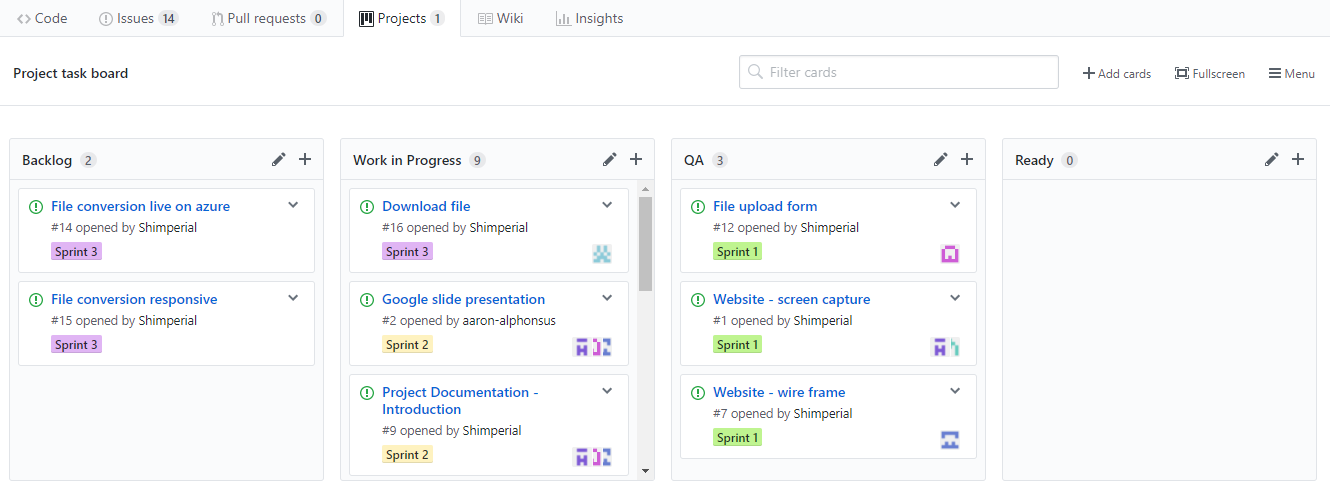
\includegraphics[width=\textwidth]{ProjectTaskBoard.png}
    \caption{Project Task Board}
    \label{fig:ProjectTaskBoard}
\end{figure}

By default, only the development team has access to the Sprint and Product 
Backlog on GitHub.  Documentation, presentations, and 
other communications provide insight into the status of the project to other interested parties. 

\subsection{Sprints}
The Senior Design I development methodology was an agile development methodology.
The features and milestones were created at the beginning of the semester, with 6 full sprints planned for the semester.\\

At the start of the Senior Design II course, the development team opted to use a Feature Driven Development (FDD) methodology.  
This decision was made primarily due to the large team size, scheduling meeting times for sprint planning and retrospective presented a challenge, as did the more rigid of the Agile methodology.\\

For a more detailed discussion of project management productivity tracking, reference \ref{sec:SprintOverview}.

\section{Proof of Concept Results}


The first semester was centered on giving the 
stakeholders a proof of concept product so that they can begin to drive the requirements
of the project in the future. The team had meetings with faculty to demo 
 VR and AR technology to prepare for integration in the classroom. At the end of the first semester, an MVP was available for demonstration. 

\section{Supporting Material}

All supporting materials have been included in Appendix \ref{ch:support}. Included is the Mobile Computing Grant which outlines SD Mine's long-term goals of this project. These goals have been used to define the direction and requirements of this project.
